%! Author = jiang-ziyang
%! Date = 22-7-1

% Preamble
\documentclass{ctexart}

% Packages
\usepackage{graphicx}
\usepackage{float}
\usepackage{subfigure}
\usepackage{amsmath}
\usepackage{amsfonts}
\usepackage{amssymb}
\usepackage{amsthm}
\usepackage{listings}
\usepackage{xcolor}
\usepackage[backref]{hyperref}
\usepackage{cite}
\usepackage{stmaryrd}
\lstset{
    basicstyle          =   \sffamily,          % 基本代码风格
    keywordstyle        =   \bfseries,          % 关键字风格
    commentstyle        =   \rmfamily\itshape,  % 注释的风格,斜体
    stringstyle         =   \ttfamily,  % 字符串风格
    flexiblecolumns,
    breaklines          =   true, %对过长的代码自动换行
    numbers             =   left,   % 行号的位置在左边
    showspaces          =   false,  % 是否显示空格,显示了有点乱,所以不现实了
    numberstyle         =   \zihao{-5}\ttfamily,    % 行号的样式,小五号,tt等宽字体
    showstringspaces    =   false,
    captionpos          =   t,      % 这段代码的名字所呈现的位置,t指的是top上面
    frame               =   lrtb,   % 显示边框
}


\title{Manderbrot Set 的生成和探索}
\author{杨泽加 \\ 统计学 3190104662}

% Document
\begin{document}
    \bibliographystyle{IEEEtran}

    \maketitle

    \begin{abstract}\
        {\kaishu 本文介绍了 Manderbrot Set 的基本信息,并以 python + Cython 提供了绘制
        Mandelbrot Set 的一种实现方式。}
    \end{abstract}
    \section{引言}\label{S1}
    \begin{tabular}{p\columnwidth}
        曼德博集合(英语:Mandelbrot set,或译为曼德布洛特复数集合)是一种在复平面上组成分形
        的点的集合,以数学家本华·曼德博的名字命名。\cite{mandelbrotWiki}\\
        Mandelbrot 集的图像展示了一个精细且无限复杂的边界,随着放大倍数的增加,
        它会显示出越来越精细的递归细节;在数学上,有人会说曼德布罗集的边界是一条分形曲线。
        Mandelbrot Set 因其美学吸引力和作为由应用简单规则而产生的复杂结构的示例而在数学之外变得流行。
        它是数学可视化、 数学美和主题最著名的例子之一。\\
    \end{tabular}
    \section{问题的背景介绍}\label{S2}
    \begin{tabular}{p\columnwidth}
        Mandelbrot 集起源于复动力学,这是 20 世纪初法国数学家 Pierre Fatou和Gaston Julia首次研究的领域。
        1978 年,罗伯特·W·布鲁克斯和彼得·马特尔斯基首次定义并绘制了这种分形,
        作为克莱因群研究的一部分。\cite{IRwinKraRB&JPM}1980 年 3 月 1 日,
        Benoit Mandelbrot在纽约约克镇高地的IBM托马斯 J. 沃森研究中心首次看到了该集合的可视化。\\
        Mandelbrot在 1980 年发表的一篇文章中研究了二次多项式的参数空间。\cite{MandelbrotScience}
        Mandelbrot 集的数学研究真正始于数学家Adrien Douady和John H. Hubbard (1985) \cite{EtudeAD&JHH}
        的工作, 他们建立了许多基本属性 , 并命名该集合以纪念 Mandelbrot 在分形几何方面的工作。\\
        1985 年 8 月的《科学美国人》的封面文章向广大读者介绍了计算 Mandelbrot 集的算法。
        封面由不来梅大学的Peitgen 、Richter 和Saupe创作。\cite{AmericanScience4A1985}\\
        Douady 和 Hubbard 的工作恰逢对复杂动力学和抽象数学的兴趣大幅增加,
        而 Mandelbrot 集的研究从此成为该领域的核心。
    \end{tabular}
    \section{数理理论}\label{S3}
    \begin{tabular}{p\columnwidth}
        Mandelbrot Set可以用复二次多项式定义:
        \begin{equation}
            \label{E1}
            f_x(z) = z^2 + c
        \end{equation}
        其中 $c$ 是一个复数参数。
        从 $z = 0$ 开始对 $f_c(z)$ 进行迭代:
        \begin{equation}
            \label{E2}
            z_{n+1} = z_n^2 + c, n = 0,1,2,\cdots
        \end{equation}
        不同的参数 $c$ 可能使序列的绝对值逐渐发散到无限大,也可能收敛到有限的区间内。
        Mandelbrot Set $\mathbf{M}$ 就是使序列不发散到无线打的所有复数 $c$ 的集合。
        下面不给出证明阐述它的一些定理。
    \end{tabular}
    \subsection{相关的定理}\label{S31}
    \newtheorem{theorem}{定理}
    \begin{theorem}\label{T1}
        若 $|c| \leqslant \frac14 $,则 $c\in\mathbf M$。
    \end{theorem}
    \begin{theorem}\label{T2}
        若 $c \in \mathbf{M}$, 则 $|c| \leqslant 2$。
    \end{theorem}
    \begin{theorem}\label{T3}
        若 $c\in \mathbf{M}$,则 $|z_n| \leqslant 2,(n=1,2,\cdots)$。
    \end{theorem}
    \section{算法}\label{S4}
    \begin{tabular}{p\columnwidth}
        由 Mandelbrot Set 的定义\autoref{S3}知其是一个无界点集。因此我们总是找一个
        具体的区间进行计算和绘制。由于计算机不可能无限迭代,我们取一个足够大的数作为最大
        迭代次数。又取一个大于等于2的正数\eqref{T3}作为逃逸限进行迭代。之后根据迭代次数为图片上色。\\
        其中,迭代区间、迭代次数、逃逸限和调色方式均会影响到图片的效果。对区间进行的点集划分
        会影响到图片的精度。
    \end{tabular}
    \section{数值算例}
    本节将展示两个区间的 Mandelbrot Set 绘图结果。
    \begin{figure}[H]
        \centering
        \subfigure[以(0.27322626, 0.595153338)为中心,边长为0.4]{
        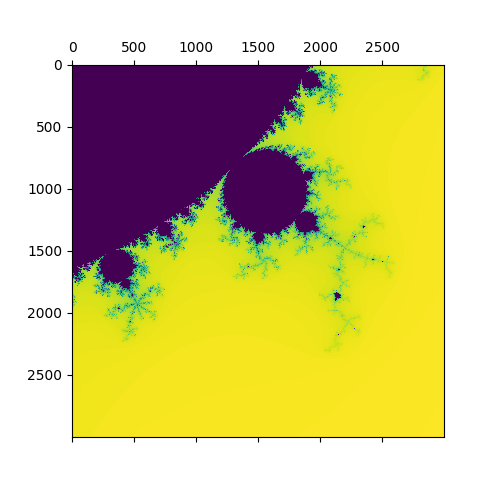
\includegraphics[width=0.4\textwidth]{mandelbrot}
        \label{Fig1}}
        \subfigure[以(0,0)为中心,边长为3]{
        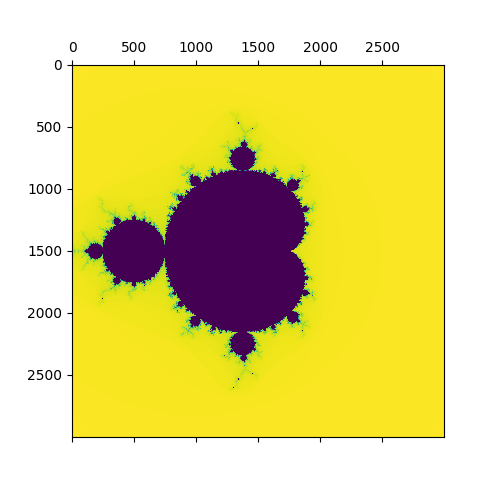
\includegraphics[width=0.4\textwidth]{mandelbrotMain}
        \label{Fig2}}
        \subfigure[以(-0.7214576, 0.2421354)为中心,边长为0.02]{
        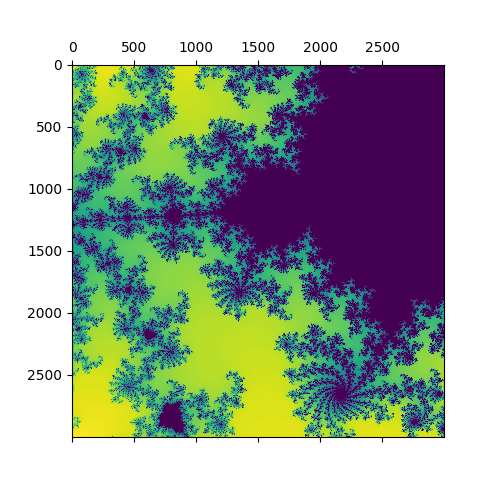
\includegraphics[width=0.4\textwidth]{mandelbrotNext}
        \label{Fig3}
        }
    \end{figure}
    \section{结论}\label{S5}
    \begin{tabular}{p\columnwidth}
        通过上述解释,我们更加清楚地理解了 Mandelbrot Set 的一些性质,也能够更加直观地感受
        到它的美感。作为一个分形图形,它的细节是异常丰富的。也希望读者可以通过调整调色模型,
        迭代次数和逃逸限来创造自己的 Mandelbrot Set 图形。
    \end{tabular}
    \bibliography{reference}
\end{document}